% !TEX TS-program = pdflatex
% !TEX encoding = UTF-8 Unicode

% This is a simple template for a LaTeX document using the "article" class.
% See "book", "report", "letter" for other types of document.

\documentclass[11pt]{article} % use larger type; default would be 10pt

\usepackage[utf8]{inputenc} % set input encoding (not needed with XeLaTeX)

%%% Examples of Article customizations
% These packages are optional, depending whether you want the features they provide.
% See the LaTeX Companion or other references for full information.

%%% PAGE DIMENSIONS
\usepackage{geometry} % to change the page dimensions
\geometry{a4paper} % or letterpaper (US) or a5paper or....
% \geometry{margin=2in} % for example, change the margins to 2 inches all round
% \geometry{landscape} % set up the page for landscape
%   read geometry.pdf for detailed page layout information

\usepackage{graphicx} % support the \includegraphics command and options

% \usepackage[parfill]{parskip} % Activate to begin paragraphs with an empty line rather than an indent

%%% PACKAGES
\usepackage{booktabs} % for much better looking tables
\usepackage{array} % for better arrays (eg matrices) in maths
\usepackage{paralist} % very flexible & customisable lists (eg. enumerate/itemize, etc.)
\usepackage{verbatim} % adds environment for commenting out blocks of text & for better verbatim
\usepackage{subfig} % make it possible to include more than one captioned figure/table in a single float
% These packages are all incorporated in the memoir class to one degree or another...

\usepackage{amsmath}
\usepackage{amssymb}
\usepackage{amsfonts}
\usepackage{amsthm}
\usepackage{varwidth}
% \usepackage{quiver}
\usepackage{esint}

\usepackage{soul} % Very fun!
\usepackage{ragged2e}
\usepackage{xcolor}
\usepackage{hyperref}
% \usepackage{asymptote}
\usepackage{twemojis}
\usepackage{gensymb}
\usepackage[super]{nth}
\usepackage{enumitem}
\usepackage{scrambledenvs}

%%% HEADERS & FOOTERS
\usepackage{fancyhdr} % This should be set AFTER setting up the page geometry
\pagestyle{fancy} % options: empty , plain , fancy
\renewcommand{\headrulewidth}{0pt} % customise the layout...
\lhead{}\chead{}\rhead{}
\lfoot{}\cfoot{\thepage}\rfoot{}

%%% SECTION TITLE APPEARANCE
\usepackage{sectsty}
\allsectionsfont{\sffamily\mdseries\upshape} % (See the fntguide.pdf for font help)
% (This matches ConTeXt defaults)

%%% ToC (table of contents) APPEARANCE
\usepackage[nottoc,notlof,notlot]{tocbibind} % Put the bibliography in the ToC
\usepackage[titles,subfigure]{tocloft} % Alter the style of the Table of Contents
\renewcommand{\cftsecfont}{\rmfamily\mdseries\upshape}
\renewcommand{\cftsecpagefont}{\rmfamily\mdseries\upshape} % No bold!

% Problems and solutions counter

\newtheorem{theorem}{Theorem}

\theoremstyle{definition}
\newtheorem{problem}{Problem}
\newtheorem{definition}{Definition}

\theoremstyle{remark}
\newtheorem*{lemma}{Lemma}

\newscrambledenv{talk}

%%% END Article customizations

%%% The "real" document content comes below...

\title{\textbf{Favorites} \\ \normalsize A compilation of problems --- Might be a draft}
\author{\texttt{asimplebeginner} (\href{https://discord.gg/mods}{Discord}) aka \texttt{TimeDependentSubset} (\href{https://artofproblemsolving.com/community/user/1281032}{AoPS})}
%\date{} % Activate to display a given date or no date (if empty),
         % otherwise the current date is printed 

\begin{document}
\maketitle

\begin{quotation}
\begin{FlushRight}
\begin{minipage}{0.9\linewidth}
\begin{FlushRight}
    \scriptsize
    you're SPAMMING!! stop SPAMMING!! all you do is SPAM!! all day, all night, every day, every night, monday, tuesday, wednesday, thursday, friday, saturday, sunday, and monday AGAIN, all you do is sit in front of the computer, stare at the computer screen, and SPAM the same five letters, ECKS OH OH KAY ESS ECKS OH OH KAY ESS, OVER and OVER and OVER AGAIN!!! PLEASE, I IMPLORE you, just look away from the computer screen!! do some pushups; solve an interesting math problem; go outside; touch some grass; get a girlfriend!!! ANYTHING!!! just STOP SPAMMING!!! PLEASE!!! just STOP!! i've NEVER seen you do ANYTHING other than SPAM the phrase X O O K S on DISCORD!!! your SPAMMING is taking up all my internet bandwidth!! i can't do ANYTHING, my computer thinks its DDOS, not a SINGLE bit of information can get through, all because of YOU and YOUR SPAMMING!!! PLEASE, just STOP SPAMMING!!! PLEASE!!!!!!!! \twemoji{sob}\twemoji{sob}\twemoji{sob}
\end{FlushRight}
\end{minipage} \\[0.5em]
\end{FlushRight}
--- \;Copypasta
\end{quotation}

About a year ago, when I was in \nth{9} grade, practicing for the city-level stage of INAMO (Indonesian Mathematical Olympiad)\footnote{Indonesians call it ``OSK Matematika''.}, I was browsing the Internet in a gloomy mood, when I decided to enter a Discord invite I was first hesitant about. It was an invite to the \href{https://discord.gg/mods}{Mathematical Olympiads Discord Server}, a (partnered) Discord server with a focus on Mathematical Olympiads, as the name implies.

There I found\footnote{...A year ago. A lot has changed over the year, and I kinda miss my early days. Hey, at least the bot works.}, along with wonderful people, the amazing volunteer-based \emph{Problem Of The Day} system held up by the server's internal bot \texttt{MODSBot}. It presented to me a myriad of problems\footnote{As of writing, \textbf{2534} problems and counting!} sourced from competitions, big and small, niche and popular; with problems easy and hard, gross and beautiful, long and short, all in the 4 flavours \emph{Algebra}, \emph{Combinatorics}, \emph{Geometry}, and \emph{Number Theory}. There I grinded, together and alone, 'till as of writing I marked \textbf{217} problems as \emph{solved}!

And now, after a year, I'm here, typing this document, and I wanna share it all. What I'm writing here is a compilation of all of the \textcolor{purple!80!black}{cool gems} I found over the year, ``favorite'' problems I find to be interesting (or rather instructive), or that I find simply funny.

This also serves as a homage to my early days in the Discord server mentioned above, and also my (as of writing, rather inactive) presence in the \emph{Art Of Problem Solving} forums\footnote{Most problems from \emph{Problem Of The Day} has discussion over at the \emph{Art Of Problem Solving} forums, and the forums has a \textbf{LOT} of cool stuff on it too!}. Hope you enjoy!

\newpage
\tableofcontents

\newpage

\section{POTD}
Every \emph{Problem Of The Day} problem (called POTDs) are numbered sequentially, starting from \textbf{POTD 1} at the \nth{26} of March 2019.

You can fetch these problems with \texttt{-fetch <potd id>}; once you're done, you can \emph{mark} the problem as solved with \texttt{-mark}. You can consult the bot with more information (\texttt{-t tutorial}).

Anyhow, POTDs have \emph{difficulty ratings}, given by the problem curator. There are also \emph{community difficulty ratings}, which you can look at (\texttt{-rating <potd id>}) or add to (\texttt{-rate <potd id>}).

I'll just include \texttt{-t diff} for reference: \\[1em]

The MODS difficulty scale is a scale ranging between 0 and 14 inclusive,  with a larger number indicating a harder problem.  All POTD questions come with a difficulty rating,  but you can add your own rating using \verb|-rate [potd] rating| or see what others think about the difficulty with \verb|-rating [potd]|.

Here are some (rough) estimations of how hard problems from competitions are:
\begin{verbatim}
DIFFICULTY (approximate)
1-4: BMO1
2-6: AMO (Australia)
3-7: BMO2
4-8: EGMO
4-10: APMO
6-11: USAMO
5-7: IMO 1/4
7-9: IMO 2/5
9-11: IMO 3/6
\end{verbatim}

And a conversion table from MODS Difficulty to MOHS:
\begin{verbatim}
d -> MOHS
5 -> 5
6 -> 10-15
7 -> 15-20
8 -> 25-30
9 -> 35
10 -> 40 (or easy 45)
11 -> 45 (or easy 50)
12 -> 50-55
\end{verbatim}

\newpage
\section{Problems}

Here lies the treasure!

Even though the title of this document is ``Favorites'', I'll also sprinkle in some problems I find instructive/introductory\footnote{A lot of overlap.}, and/or funny/interesting.

This is divided into the 4 flavors/genres\footnote{There's some overlap between them, one I like is Combinatorial Algebra (Algebra and Combinatorics)}, and in each I'll try to order the problems based off how much I like it in general. It's imperfect, though, and I really don't want to think about ordering these problems either.

To make it clear, \textbf{I'm not ordering them based on difficulty.} If you're stuck (and you're \emph{sure} stuck) on a problem, try to ask (ask \emph{real people, please.}), or you can leave the problem for later.\footnote{These problems personally took me around \textbf{1 hour - 4 hours} each (well except for a select few others). They were satisfying, though.} I'll also include some \emph{talk} about the problems, but they're more closer to my \emph{commentary} of the problem than a \emph{hint}.\footnote{One of the lessons I'm still learning about today is to think twice before asking for a hint; that's why I'll try to keep the "talks" not as helpful. When you do actually read the commentary, try to explore what it means! If you really want hints though, go ask around \texttt{:)}}

Most importantly, \textcolor{orange}{\textbf{have fun!}}

\subsection{\texttt{A} Algebra}
\setcounter{problem}{0}

\begin{problem}[\href{https://artofproblemsolving.com/community/c6h3627009p35569626}{\texttt{Deathwing}'s inequality}]
    Let \(b_1,b_2,\ldots, b_n\) be a sequence of nonnegative reals satisfying \(b_1 \geq b_2 \geq b_3 \geq \dots \geq b_n\). Determine the largest real constant \(c\) such that for any sequences of real numbers \(a_1, a_2, a_3, \ldots\) satisfying \(a_i + a_j \geq a_{i + j}\) for all positive integers \(i\leq j\), the inequality
    \[a_1b_1+a_2b_2+\cdots + a_nb_n \geq c a_{n+1}\]
    holds.
    \begin{talks}
        \begin{talk}
            Felt like combing hair tbh.
        \end{talk}
        \begin{talk}
            \texttt{Deathwing} is one of my friends I met during OSN/INAMO. Hiiiiiiiiii \texttt{>w<}
        \end{talk}
    \end{talks}
\end{problem}

\begin{problem}[POTD 557]
    Consider a function \(f: \mathbb{R}^2 \to \mathbb{R}^2\) which sends points in the Euclidean plane to points in the Euclidean plane.
    Define by \(d(X, Y)\) the Euclidean distance between points \(X\) and \(Y\).
    Suppose that for each pair of points \(X, Y \in \mathbb{R}^2\) the points \(f(X)\) and \(f(Y)\) satisfy the inequality
    \[d(f(X), f(Y)) \leq 0.999 \hspace{0.1cm} d(X, Y)\]
    Show that there is a unique point \(P \in \mathbb{R}^2\) that satisfies \(f(P) = P.\)
    \begin{talks}
        \begin{talk}
            Apparently I heard that this problem could be generalized to any (complete) metric spaces, whatever that means...
        \end{talk}
        \begin{talk}
            This is an example of a bizzare type of problem that appears in POTD. In the spreadsheet it has the tag \texttt{X}, aka "Outside IMO Scope". There are other examples of this, but most of them are above my level...

            Yeah you definitely don't need to study metric spaces or topology to train for olympiads \twemoji{skull}
        \end{talk}
    \end{talks}
\end{problem}

\begin{problem}[POTD 958]
    Let \(X, Y\) be subsets of \(\mathbb{R}^2\). Say a function \(f : X \to Y\) is continuous if for any \(\varepsilon > 0\), there exists a \(\delta > 0\) such that for any \(x_1, x_2 \in X\) with \(|x_1 - x_2| < \delta\) we have \(|f(x_1) - f(x_2)| < \varepsilon\). Say \(X\) and \(Y\) are homemorphic if there exists a continuous bijection \(f : X \to Y\) such that \(f^{-1}\) is continuous. Is \(\mathbb{R}^2\) homeomorphic to \(\mathbb{R}^2 \backslash \{(0,0)\}\)?
    \begin{talks}
        \begin{talk}
            This is firmly outside the scope of olympiads.
        \end{talk}
        \begin{talk}
            Lucky I ever solved this, because I've read the related material (although only a little bit). I should maybe seriously learn stuff like this someday... (I'm lazy \twemoji{melting face})
        \end{talk}
        \begin{talk}
            For how I solved this, look up ``fundamental groups''.
        \end{talk}
    \end{talks}
\end{problem}

\begin{problem}[POTD 1334]
    Find all functions \(f:\mathbb{R}\rightarrow\mathbb{R}\) such that for all \(x,y\in\mathbb{R}\) the following equality holds \[ f(\left\lfloor x\right\rfloor y)=f(x)\left\lfloor f(y)\right\rfloor \] where \(\left\lfloor a\right\rfloor \) is greatest integer not greater than \(a\).
    \begin{talks}
        \begin{talk}
            This is a subgenre called \emph{Functional Equations}. Most of the time you'll have statements involving a function \(f: A \rightarrow B\) from domain \(A\) to codomain \(B\), some variables and some constants. The goal is to find all functions \(f\) that satisfy some property. I recommend you (the reader) to look into these types of problems, they're fun \texttt{:D}
        \end{talk}
    \end{talks}
\end{problem}

\begin{problem}[POTD 1895]
    Prove that every positive integer can be written as a finite sum of distinct integral powers of the golden ratio.
    \begin{talks}
        \begin{talk}
            Fun type of induction! Usually you'll have \(P(x) \Rightarrow P(x+1)\) for some logical predicate \(P\), but this time you'll have to get a bit more creative \texttt{:D}
        \end{talk}
        \begin{talk}
            I'll save you the trouble:
            \[\varphi^2 = \varphi + 1\]
        \end{talk}
    \end{talks}
\end{problem}

\begin{problem}[POTD 844]
    Let \(S\) be the set of all infinite positive integer sequences. We say that two sequences in \(S\) are \emph{separated} if, for all positive integers \(n\), the \(n\)th term in the first sequence is distinct from the \(n\)th term in the second sequence. \\

    Find all functions \(f:S\to \mathbb{Z}^+\) such that:
    \begin{enumerate}[label=(\roman*)]
        \item \(f(s_1)\neq f(s_2)\) for any two separated sequences \(s_1,s_2\in S\);
        \item For any constant sequence \(s=(c,c,c,\dots)\in S\), we have \(f(s)=c\). 
    \end{enumerate}
    \begin{talks}
        \begin{talk}
            A sequence can be interpreted as a function \(\mathbb{Z}^+ \rightarrow \mathbb{Z}^+\), so in this case this FE has the funny type signature
            \[f: (\mathbb{Z}^+ \rightarrow \mathbb{Z}^+) \rightarrow \mathbb{Z}^+\]
        \end{talk}
    \end{talks}
\end{problem}

\subsection{\texttt{C} Combinatorics}
\setcounter{problem}{0}

\begin{problem}[POTD 2132]
    Let \(f \colon \mathbb{R} \to \mathbb{R}\) be a bijective function. Does there always exist an infinite number of functions \(g \colon \mathbb{R} \to \mathbb{R}\) such that \(f(g(x))=g(f(x))\) for all \(x \in \mathbb{R}\)?
    \begin{talks}
        \begin{talk}
            This has been the most liked problem of mine until recently \twemoji{face with open mouth}
        \end{talk}
        \begin{talk}
            This was my personal introduction to the (really cool!) \emph{sub}subgenre \emph{Arrow FE}, aka \emph{Functional Equations} combined with \emph{Graph Theory}.

            The problem itself was intuitive; I solved this problem almost instantaneously, though writing it up took me \emph{all day...} The same idea behind this problem can be echoed through the entire subgenre (at least what I'm aware of), but in my opinion this problem distills/presents the idea in its bare form really well.
        \end{talk}
    \end{talks}
\end{problem}

\begin{problem}[POTD 1621]
    Let \(\mathbb{N}\) be the set of positive integers. Determine all positive integers \(k\) for which there exist functions \(f : \mathbb{N} \to \mathbb{N}\) and \(g : \mathbb{N} \to  \mathbb{N}\) such that \(g\) assumes infinitely many values and such that \[f^{g(n)}(n) = f(n) + k\] holds for every positive integer \(n\).
    \begin{talks}
        \begin{talk}
            Have fun constructing \texttt{:)} A diagram really helps in these dire times.
        \end{talk}
    \end{talks}
\end{problem}

\begin{problem}[POTD 320]
    On an infinite square grid we place finitely many \emph{cars}, which each occupy a single cell and face in one of the four cardinal directions. Cars may never occupy the same cell. It is given that the cell immediately in front of each car is empty, and moreover no two cars face towards each other in the same row or column (no right-facing car is to the left of a left-facing car within a row, etc.). In a \emph{move}, one chooses a car and shifts it one cell forward to a vacant cell. Prove that there exists an infinite sequence of valid moves using each car infinitely many times. 
    \begin{talks}
        \begin{talk}
            You should \emph{really} avoid spoilers for this problem in particular. You'll regret it.
        \end{talk}
        \begin{talk}
            Took me 4 hours. Take your time.
        \end{talk}
        \begin{talk}
            Very funny problem. The intended solution takes up \(\frac{1}{2}\) of a page.
        \end{talk}
    \end{talks}
\end{problem}

\begin{problem}[POTD 1874]
    Let \(n\) be a positive integer. A \textit{Japanese triangle} consists of \(1 + 2 + \dots + n\) circles arranged in an equilateral triangular shape such that for each \(i = 1\), \(2\), \(\dots\), \(n\), the \(i^{th}\) row contains exactly \(i\) circles, exactly one of which is coloured red. A \textit{ninja path} in a Japanese triangle is a sequence of \(n\) circles obtained by starting in the top row, then repeatedly going from a circle to one of the two circles immediately below it and finishing in the bottom row. Here is an example of a Japanese triangle with \(n = 6\), along with a ninja path in that triangle containing four red circles.\footnote{Thanks for the diagram, Celestia!}

    \begin{center}
        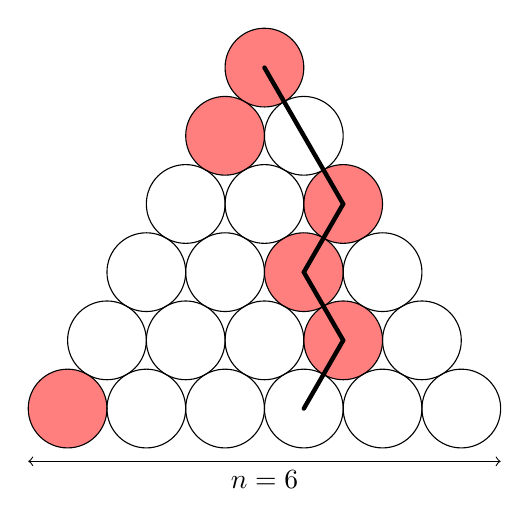
\begin{tikzpicture}
            \def\r{0.5}
            \def\s{5}

            \foreach \i in {0,...,\s}{
                \foreach \j in {0,...,\i}{
                    \ifnum\i<2 \ifnum\j=0
                        \fill[color=red,opacity=0.5] (\j*2*\r-\i*\r,-\i*1.732*\r) circle (\r);
                    \fi \fi
                    \ifnum4>\i>1 \ifnum\j=2
                        \fill[color=red,opacity=0.5] (\j*2*\r-\i*\r,-\i*1.732*\r) circle (\r);
                    \fi \fi
                    \ifnum\i=4 \ifnum\j=3
                        \fill[color=red,opacity=0.5] (\j*2*\r-\i*\r,-\i*1.732*\r) circle (\r);
                    \fi \fi
                    \ifnum\i=5 \ifnum\j=0
                        \fill[color=red,opacity=0.5] (\j*2*\r-\i*\r,-\i*1.732*\r) circle (\r);
                    \fi \fi
                    \draw (\j*2*\r-\i*\r,-\i*1.732*\r) circle (\r);
                }
            }

            \draw[ultra thick,line cap=round] (0, 0) -- (2*\r, -1.732*2*\r);
            \draw[ultra thick,line cap=round] (2*\r, -1.732*2*\r) -- (1*\r, -1.732*3*\r);
            \draw[ultra thick,line cap=round] (1*\r, -1.732*3*\r) -- (2*\r, -1.732*4*\r);
            \draw[ultra thick,line cap=round] (2*\r, -1.732*4*\r) -- (1*\r, -1.732*5*\r);
            \draw[<->] (-6*\r, -10*\r) -- (6*\r, -10*\r) node[midway,below] {$n=6$};

        \end{tikzpicture}
    \end{center}

    In terms of \(n\), find the greatest \(k\) such that in each Japanese triangle there is a ninja path containing at least \(k\) red circles.
\end{problem}

\begin{problem}[POTD 1718]
    Let \(2^{[n]}\) denote the set of subsets of \([n] := \{1,2,\ldots,n\}\). Find all functions \(f:2^{[n]} \rightarrow 2^{[n]}\) which satisfy \[|A \cap f(B)| = |B \cap f(A)|\] for all subsets \(A\) and \(B\) of \([n]\).
    \begin{talks}
        \begin{talk}
            I'm not even sure why they labelled this as \texttt{CA} instead of just \texttt{C}. I mean, look at it, the domain and codomain are \emph{sets of subsets!}
        \end{talk}
    \end{talks}
\end{problem}

\begin{problem}[POTD 1566]
    Prove that, for any positive integer \(n\), there are equally many ways to partition a set of \(n\) objects into piles of distinct sizes as ways to partition the set into piles of odd sizes.
    \begin{talks}
        \begin{talk}
            I remember the time during my junior highschool days when my tutor sent me this as "homework" (there's no deadline). I occasionally thought about the problem for about \textbf{3 months} before I stumbled upon the solution while reading something on LibreTexts.

            That was fun. Good intro for \emph{Generating Functions} also.
        \end{talk}
        \begin{talk}
            There's actually a clever bijective solution (no generating functions). Broke my heart when I saw it.
        \end{talk}
    \end{talks}
\end{problem}

\subsection{\texttt{G} Geometry}
\setcounter{problem}{0}

I'll admit, I haven't practiced enough Geometry\footnote{I have severe Geometry skill issue send help} to have good enough taste. Please send problems.

Oh well, I could use some filler.

\begin{problem}[POTD 1524]
    The incircle \(\omega\) of a triangle \(ABC\) is tangent to sides \(BC\), \(CA\) and \(AB\) at \(D\), \(E\) and \(F\) respectively. Let \(M\) be the midpoint of \(EF\). Let lines \(AD\) and \(EF\) intersect at \(P\). Let the circumcircle of triangle \(AMP\) meets \(AB\) and \(AC\) again at \(X\) and \(Y\) respectively. Let the tangents to the circumcircle of triangle \(AXY\) at \(X\) and \(Y\) meet at a point \(Z\).
    \\ Prove that the circle with centre \(Z\) that goes through \(M\) is orthogonal to the circumcircle of triangle \(AEF\).
    \begin{talks}
        \begin{talk}
            This problem's made by a friend. Thanks Atavic/Nolao! (He's called \verb|AlephG_64| on AoPS.)
        \end{talk}
    \end{talks}
\end{problem}

\begin{problem}[Cevian Nest]
    In the plane of a triangle \(\triangle ABC\).

    Let \(A' \in BC\), \(B' \in CA\), \(C' \in AB\) such that \(AA'\), \(BB'\), \(CC'\) concur.

    Let \(A'' \in B'C'\), \(B'' \in C'A'\), \(C'' \in A'B'\) such that \(A'A''\), \(B'B''\), \(C'C''\) concur.

    Prove that the lines \(AA''\), \(BB''\), \(CC''\) concur.
    \begin{talks}
        \begin{talk}
            Cool use of the \(\prod\) notation. I rarely see those outside of ineq...
        \end{talk}
    \end{talks}
\end{problem}

\begin{problem}[This was from my homework smh]
    Let \(M\) and \(N\) be distinct points on the plane of \(\triangle ABC\) such that
    \[AM : BM : CM = AN : BN : CN\]
    Prove that \(M - N - O\) (\(M\), \(N\) and \(O\) are collinear) where \(O\) is the circumcenter of \(\triangle ABC\).
    \begin{talks}
        \begin{talk}
            A \emph{locus} is a set of points that satisfy some property. Usually they'll become a nice shape/curve. If you graph the set of points \(X\) such that \(AM : BM = AX : BX\), what do they look like?
        \end{talk}
    \end{talks}
\end{problem}

\begin{problem}[Simon line gaming. Also from my homework]
    Let \((ABCD)\) be a cyclic quadrilateral.
    \begin{enumerate}[label=(\alph*)]
        \item Let \(D_A\) be the foot of the perpendicular from \(D\) to \(BC\), that is, \(D_A \in BC\) with \(D_AD \perp BC\). Define \(D_B \in AC\) and \(D_C \in AB\) similarly. Show that \(D_A - D_B - D_C\) (\(D_A\), \(D_B\), \(D_C\) are collinear.)
        \item Let \(\ell_D\) be the line \(D_A - D_B - D_C\), and define \(\ell_A\), \(\ell_B\), \(\ell_C\) similarly. Prove that \(\ell_A\), \(\ell_B\), \(\ell_C\), \(\ell_D\) concur at one point.
    \end{enumerate}
    \begin{talks}
        \begin{talk}
            I can see you trying to draw \(A_B\), \(A_C\), \(A_D\), \(B_A\), \(B_C\), \(B_D\), \(C_A\), \(C_B\), \(C_D\), \(D_A\), \(D_B\), and \(D_C\)...
        \end{talk}
        \begin{talk}
            Apparently this is called "Config Geo", geometry problems derived from a variety of configurations. This problem in particular is from the \emph{Orthocenter} configuration.

            I'm not qualified to talk about this, go ask someone better than me in geometry \texttt{:)} (It's a low bar.)
        \end{talk}
    \end{talks}
\end{problem}

\begin{problem}[Brocard's Theorem (one part of it)]
    Let \(ABCD\) be a cyclic quadrilateral with circumcenter \(O\). Let \(P = AC \cap BD\), \(Q = AD \cap BC\), \(R = AB \cap CD\) (take points of infinity if the lines are parallel).

    Prove that \(O\) is the orthocenter of \(\triangle PQR\).
    \begin{talks}
        \begin{talk}
            There's more to this theorem. You can prove that \(QR\) is the polar of \(P\), i.e. when you take \(P' \in PO\) such that \(OP \cdot OP'\), then \(\angle QP'P = \angle RP'P = 90 \degree\). Similarly goes for the others.
        \end{talk}
    \end{talks}
\end{problem}

\begin{problem}[POTD 428]
    Two chords, \(A C\) and \(B D\), in a circle with centre \(O\), intersect at \(E .\) The circumcircles of triangles \(E A B\) and \(E C D\) intersect again at \(F .\) Prove \(O F\) is perpendicular to \(E F\).
    \begin{talks}
        \begin{talk}
            If you squint hard enough, this is equivalent to a part of Brocard's Theorem.
        \end{talk}
    \end{talks}
\end{problem}

\begin{problem}[Also from my homework]
    Let \(ABCD\) be a quadrilateral with a tangent incircle \(\Gamma\), such that \(\Gamma\) is tangent to \(AB\) at \(X_{AB}\), tangent to \(BC\) at \(X_{BC}\), tangent to \(CD\) at \(X_{CD}\), and tangent to \(DA\) at \(X_{DA}\). Prove that \(AC\), \(BD\), \(X_{AB} X_{CD}\), \(X_{BC} X_{DA}\) are concurrent.
    \begin{talks}
        \begin{talk}
            If you squint hard enough, you can prove Brocard's Theorem from this.
        \end{talk}
    \end{talks}
\end{problem}

\subsection{\texttt{N} Number Theory}
\setcounter{problem}{0}

\begin{problem}[POTD 1782]
    Let \(\mathbb N\) denote the set of positive integers. A function \(f\colon\mathbb N\to\mathbb N\) has the property that for all positive integers \(m\) and \(n\), exactly one of the \(f(n)\) numbers
    \[f(m+1),f(m+2),\ldots,f(m+f(n))\]is divisible by \(n\). Prove that \(f(n)=n\) for infinitely many positive integers \(n\).
    \begin{talks}
        \begin{talk}
            They call me weird because I use formal logic notation all over the place \texttt{:>}
        \end{talk}
    \end{talks}
\end{problem}

\begin{problem}[POTD 831]
    Find all integers \(n \ge 2\) for which there exists an integer \(m\) and a polynomial \(P(x)\) with integer coefficients satisfying the following three conditions:
    \begin{itemize}
        \item \(m > 1\) and \(\gcd(m,n) = 1\);
        \item the numbers \(P(0)\), \(P^2(0)\), \(\ldots\), \(P^{m-1}(0)\) are not divisible by \(n\); and
        \item \(P^m(0)\) is divisible by \(n\).
    \end{itemize}
    Here \(P^k\) means \(P\) applied \(k\) times, so \(P^1(0) = P(0)\), \(P^2(0) = P(P(0))\), etc.
    \begin{talks}
        \begin{talk}
            Cool solution set! Also, this is (in my opinion) a heavy application of \emph{Arrow FE}.
        \end{talk}
    \end{talks}
\end{problem}

\begin{problem}[POTD 2104]
    Let \(P(x)\) be a polynomial of degree \(n > 1\) with integer coefficients and let \(k\) be a positive integer. Consider the polynomial\[ Q(x) = P(P(\dots P(P(x)) \dots )) \] where \(P\) occurs \(k\) times. Prove that there are at most \(n\) integers \(t\) such that \(Q(t) = t\).
\end{problem}

\begin{problem}[POTD 627]
    Consider a sequence \(a_1, a_2, \dots \) of non-zero integers such that \(a_{m + n} \mid a_{m} - a_{n}\) for all \(m, n \in \mathbb{N}.\)
    \begin{enumerate}[label=(\alph*)]
        \item Show that the sequence can be unbounded.
        \item Do there necessarily exist \(i \neq j\) such that \(a_i = a_j\)?
    \end{enumerate}
    \begin{talks}
        \begin{talk}
            Saw someone crashing out over this. Personally, I don't see what's wrong with this problem \texttt{:')}
        \end{talk}
    \end{talks}
\end{problem}

\begin{problem}[POTD 1956]
    Prove that, for any positive integers \(a,b,c\), there is a positive integer \(k\) such that \[\gcd(a^k+bc,b^k+ac,c^k+ab)>1\]
\end{problem}

\begin{problem}[POTD 1972]
    Determine all pairs \((a,b)\) of positive integers for which there exist positive integers \(g\) and \(N\) such that \[\gcd (a^n+b,b^n+a)=g\]holds for all integers \(n\geqslant N.\) (Note that \(\gcd(x, y)\) denotes the greatest common divisor of integers \(x\) and \(y.\))
\end{problem}

\begin{problem}[POTD 711]
    We say that a set \(S\) of integers is rootiful if, for any positive integer \(n\) and any \(a_0, a_1, \cdots, a_n \in S\), all integer roots of the polynomial \(a_0+a_1x+\cdots+a_nx^n\) are also in \(S\). Find all rootiful sets of integers that contain all numbers of the form \(2^a - 2^b\) for positive integers \(a\) and \(b\).
\end{problem}

\begin{problem}[POTD 2321]
    Determine all sequences \(a_1, a_2, \dots\) of positive integers such that for any pair of positive integers \(m\leqslant n\), the arithmetic and geometric means
    \[ \frac{a_m + a_{m+1} + \cdots + a_n}{n-m+1}\quad\text{and}\quad (a_ma_{m+1}\cdots a_n)^{\frac{1}{n-m+1}}\]
    are both integers.
    \begin{talks}
        \begin{talk}
            No, just because Arithmetic Mean is mentioned doesn't mean it's an arithmetic sequence. \texttt{XD}
        \end{talk}
    \end{talks}
\end{problem}

\begin{problem}[I forgot the source]
    The positive integers \(a_1\), \(a_2\), \(a_3\), \(\dots\), all not exceeding \(1988\), form a sequence that satisfies the following condition: If \(m\) and \(n\) are positive integers, then \(a_m + a_n\) are divisible by \(a_{m+n}\). Prove that this sequence is periodic from some point onwards.
    % \begin{talks}
    %     \begin{talk}
    %     \end{talk}
    % \end{talks}
\end{problem}

\subsection{Auxiliary/Other problems}
\setcounter{problem}{0}

\begin{problem}[POTD 1362, genre \texttt{ACN}]
    Let \(n \geqslant 100\) be an integer. Ivan writes the numbers \(n, n+1, \ldots, 2 n\) each on different cards. He then shuffles these \(n+1\) cards, and divides them into two piles. Prove that at least one of the piles contains two cards such that the sum of their numbers is a perfect square.
    \begin{talks}
        \begin{talk}
            As of writing, this is the only unique \texttt{d7 ACN} on the POTD spreadsheet!
        \end{talk}
    \end{talks}
\end{problem}

\begin{problem}[POTD 45, (personal opinion) genre \texttt{CN}]
    Let \(p \geq 2\) be a prime number.
    Eduardo and Fernando play the following game making moves alternately: in each move, the current player chooses an index \(i\) in the set \(\{0,1,\dots,p-1 \}\) that was not chosen before by either of the two players and then chooses an element \(a_i\) of the set \(\{0,1,2,3,4,5,6,7,8,9\}\).
    Eduardo has the first move. The game ends after all the indices \(i \in \{0,1,\dots,p-1\}\) have been chosen. Then the following number is computed:
    \[M = a_0 + 10\cdot a_1 + \dots + 10^{p-1} \cdot a_{p-1} = \sum_{j=0}^{p-1} a_j \cdot 10^j.\]
    The goal of Eduardo is to make the number \(M\) divisible by \(p\), and the goal of Fernando is to prevent this. Prove that Eduardo has a winning strategy.
\end{problem}

\newpage

\section{Talk/Discussion/Commentary}

\printtalk

\newpage
\section*{After the dust settles}
\setcounter{problem}{0}

\hfill

\emph{Why do I hear boss music}

\vfill

\begin{figure}[h]
    \begin{Center}
        \begin{minipage}{0.6\linewidth}
            \begin{problem}[\href{https://artofproblemsolving.com/community/c6h3780559p37328805}{\textcolor{green!40!black}{\textbf{Solved as of \nth{2} of April 2026}}}] \hfill \\
                Are there any functions \(f: \mathbb{N} \to \mathbb{N}\) such that
                \[f(f(n)) = 2\varphi(n)\]
                for all \(n \in \mathbb{N}\), where \(\varphi\) is Euler's totient function?
            \end{problem}
        \end{minipage}
    \end{Center}
\end{figure}

\vfill

\end{document}
